\documentclass[11pt,fleqn]{article}
\usepackage{../cs188,latexsym,epsf, amsmath,amsfonts,graphicx,url}
\lecture{6}
\def\title{Note \the\lecturenumber}
\begin{document}
\maketitle


\iffalse
\documentclass[11pt,fleqn]{article}
\usepackage{latexsym,epsf,amsmath,amsfonts,graphicx,url}

\title{Note 6 (alpha)}

\newcommand{\F}{\mathbb{F}}
\newcommand{\Z}{\mathbb{Z}}
\newcommand{\Q}{\mathbb{Q}}
\newcommand{\R}{\mathbb{R}}
\newcommand{\C}{\mathbb{C}}

\begin{document}

\maketitle
\fi

\section*{Probabilistic Inference}

In artificial intelligence, we often want to model the relationships between various nondeterministic events. If the weather predicts a 40\% chance of rain, should I carry my umbrella? How many scoops of ice cream should I get if the more scoops I get, the more likely I am to drop it all? If there was an accident 15 minutes ago on the freeway on my route to Oracle Arena to watch the Warriors' game, should I leave now or in 30 minutes? All of these questions (and innumerable more) can be answered with \textbf{Probabilistic Inference}.

We're assuming that you've learned the foundations of probability in CS70, so these notes will not review basic concepts of probability like PDFs, conditional probabilities, independence, and conditional independence.

In previous sections of this class, we modeled the world as existing in a specific state that is always known. For the next several weeks, we will instead use a new model where each possible state for the universe has its own probability. For example, we might build a weather model, where the state consists of the season, temperature and weather. Our model might say that $P(winter, 35^\circ, cloudy) = 0.00023$. This number represents the probability of the specific outcome that it is winter, 35 degrees, and cloudy.

More precisely, our model is a \textbf{joint distribution}, i.e. a table of probabilities which captures the likelihood of each possible \textbf{outcome}, also known as an \textbf{assignment}. As an example, consider the table below:


\begin{center}	
	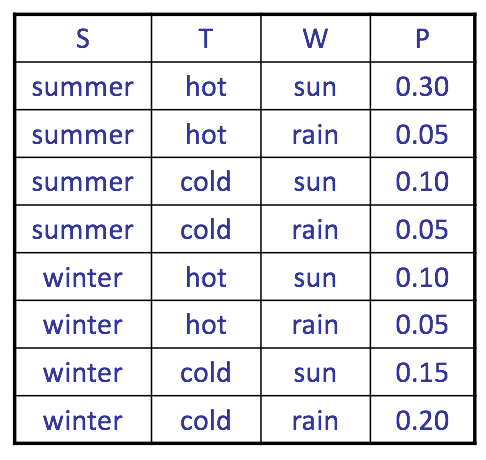
\includegraphics[height=6cm]{img/pdf_example}
\end{center}

This model allows us to answer questions that might be of interest to us, for example:

\begin{itemize}
\item What is the probability that it is sunny? $P(w = sunny)$
\item What is the probability distribution for the weather, given that we know it is winter? $P(W | s = winter)$
\item What is the probability that it is winter, given that we know it is rainy and cold? $P(s = winter | t = cold, w = rain)$
\item What is the probability distribution for the weather and season give that we know that it is cold? $P(S, W | t = cold)$
\end{itemize}

Given a joint PDF, we can trivially perform compute any desired probablity $P(Q_1...Q_k|e_1...e_k)$ using a simple intuitive procedure known as \textbf{Inference by Enumeration}. In this procedure, we collect all the rows consistent with the evidence available (i.e. $e_1...e_k$, sum out all the hidden variables (i.e. all variables for which we do not have evidence), and finally normalize the table so that it is a probability distribution (i.e. values sum to 1).

For example, if we wanted to compute $P(W | s = winter)$, we'd select the four rows where s is winter, then sum out the T variable, yielding the two row table where $P(w = sun | s = winter) = 0.5$ and $P(w = rain | s = winter) = 0.5$.

So long as we have the joint PDF table, inference by enumeration (IBE) can be used to compute any desired probablity, even for multiple query variables $Q_1...Q_k$.

\section*{Bayes Nets (Representation)}

While IBE can compute probabilities for any query we might desire, representing an entire joint distribution in the memory of a computer is impractical for real problems - if each of $n$ variable we wish to represent can take on $d$ possible values (it has a \textbf{domain} of size $d$), then our joint distribution table will have $d^n$ entries! 

Bayes nets avoid this issue by taking advantage of the idea of conditional probability. Rather than storing information in a giant table, it is instead distributed across a large number of smaller local probability tables along with a \textbf{directed acyclic graph} which captures the relationships between variables. 

Specifically, each node in the graph represents a single random variable. Arrows in the graph represent conditional independent relationships. \textbf{A node is conditionally independent of all of its non-descendants in the graph given all of its parents}. Thus, if we have a node representing variable Q, we store $P(Q | X_1, X_2, ..., X_N)$, where $X_1, ..., X_N$ are the parents of Q.

As an example of a Bayes Net, consider a model where we have five binary random variables described below:

\begin{itemize}
\item B: Burglary occurs.
\item A: Alarm goes off.
\item E: Earthquake occurs.
\item J: John calls.
\item M: Mary calls.
\end{itemize}

Assume the alarm can go off if either a burglary or an earthquake occurs, and that Mary and John will call if they hear the alarm. In this case, we can represent the natural conditional independences with the graph shown below.

\begin{center}	
	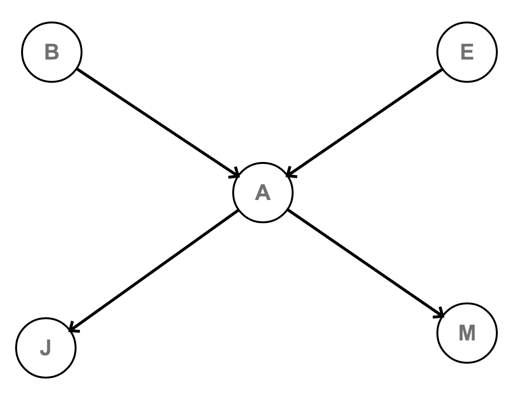
\includegraphics[height=5cm]{img/alarm_model}
\end{center}

Models capture a way the world works - they are always a simplification -
all models are wrong, but some will still be useful for solving real problems in the real world. They may may not account for every variable or even every interaction between variables.

More formally, we say that a Bayes Net consists of:
\begin{itemize}
\item A directed acyclic graph of nodes, one per variable X.
\item A conditional distribution for each node $P(X | A_1 ... A_n)$, where $A_i$ is the ith parent of X, stored as a \textbf{conditional probability table} or CPT. Each CPT has $n+1$ rows.
\end{itemize}

Given all of the CPTs for a graph, we can calculate the probability of a given assignment using the chain rule: $P(x_1, x_2, ..., x_n) = \prod_{i=1}^n{x_i | parents(X_i)}$. 

For the alarm model above, we might calculate the probability of one event as follows: $P(-b, -e, +a, +j, -m) = P(-b) \cdot P(-e) \cdot P(+a | -b, -e) \cdot P(+j | +a) \cdot P(-m | +a)$.

This works because of the conditional indepences given by the graph. Specifically, we rely on the fact that $P(x_i | x_1, ..., x_{i-1}) = P(x_i | parents(X_i))$. Or in other words, that the probability of a specific value of $X_i$ depends only on the values assigned to $X_i$'s parents.

While it is most natural to assign arrows in a Bayes Net in the same direction as causality, e.g. $earthquake \rightarrow alarm$, the direction of the arrows does not change the space of possible distributions represented by the Bayes Net. That is, if you flip an arrow, it is possible to pick new values for the CPTs such that the joint distribution is unchanged. Or stated differently: Our model is ultimately a joint distribution over all variables. The direction of the arrows does not affect which values are possible in the joint table, though the absence of arrows may restrict the possible values for the joint table, e.g. if there are no arrows, the values in the joint PDF table will need to reflect the fact that all variables are independent.

\section*{Bayes Nets (Inference)}

Inference is the process of calculating the joint PDF for some set of query variables based on some set of observed variables. We can solve this problem naively by forming the joint PDF and using Inference by Enumeration as described above. This requires creation and iteration over an exponentially large table.

An alternate approach is to \textbf{eliminate} variables one by one. To eliminate a variable X, we: 

\begin{itemize}
\item Join (multiply together) all factors involving X.
\item Sum out X.
\end{itemize}

For example, suppose we have a model as shown below, where T, C, S, and E can take on binary values, as shown below. Here, T represents the chance that an adventurer takes a treasure, C represents the chance that a cage falls on the adventurer given that he takes the treasure, E represents the chance that snakes are released if an adventurer takes the treasure, and E represents the chance that the adventurer escapes given information about the status of the cage and snakes.

\begin{center}	
	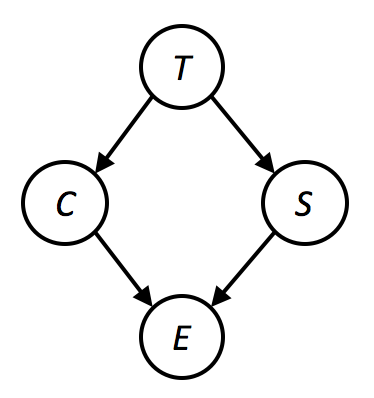
\includegraphics[height=5cm]{img/TCSE_model.png}
\end{center}

In this case, we have the factors $P(T)$, $P(C|T)$, $P(S|T)$, and $P(E|C, S)$. Suppose we want to calculate $P(T | +e)$. The naive approach would be to form the 16 row joint PDF $P(T, C, S, E)$, select only the rows corresponding to +e, then summing out C and S and finally normalizing. 

The alternate approach is to eliminate C, then S, one variable at a time. We'd proceed as follows:

\begin{itemize}
\item Join (multiply) all the factors involving C, forming $P(C, +e | T, S) = P(C|T) \cdot P(+e|C, S)$. 
\item Sum out C form this new factor, leaving us with a new factor $P(+e | T, S)$. 
\item Join all factors involving S, forming $P(+e, S | T) = P(S|T) \cdot P(+e | T,S)$.
\item Sum out S, yielding $P(+e | T)$.
\end{itemize}

Once we have $P(+e|T)$, we can easily compute $P(T|+e)$. For a more thorough working out of the example, see lecture 15.

While this process is more involved from a conceptual point of view, the maximum size of any factor generated is only 8 rows instead of 16 as it would be if we formed the entire joint PDF.

An alternate way of looking at the problem is to observe that the calculation of $P(+e, T)$ can either be done, as it is in Inference by Enumeration, as follows:

$\sum_s{\sum_c{P(T)P(s|T)P(c|T)P(+e|c,s)}}$

Variable elimination is equivalent to calculating $P(+e, T)$ as follows:

$P(T)\sum_s{P(s|T)\sum_e{P(c|T)P(+e|c,s)}}$

\section*{Bayes Nets (Sampling)}

An alternate approach for probabilistic reasoning is to implicitly calculate the probabilities for our query by simply counting samples.

For example, suppose we wanted to calculate $P(T | +e)$. If we had a magic machine that could generate samples from our distribution, we could collect all samples for which the adventurer escapes the maze, and then compute the fraction of those escapes for which the adventurer also took the treasure. Put differently, if we could run simulations of say, million of adventurers, we'd easily be able to compute any inference we'd want.

Given a Bayes Net model, we can easily write a simulator. For example, consider the CPTs given below for the simplified model with only two variables T and C.

\begin{center}	
	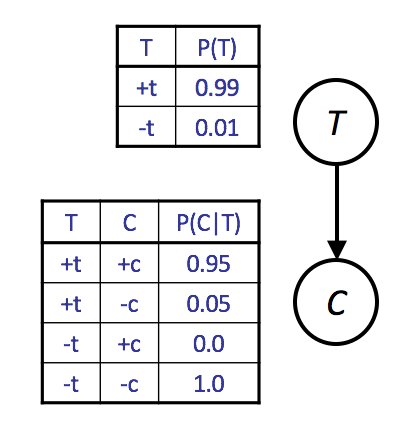
\includegraphics[height=5cm]{img/tc_model.png}
\end{center}

A simple simulator in Python would be as follows:

\begin{verbatim}
import random

def get_t():
	if random.random() < 0.99:
		return True
	return False

def get_c(t):
	if t and random.random() < 0.95:
		return True
	return False

def get_sample():
	t = get_t()
	c = get_c(t)
	return [t, c]
\end{verbatim}

We call this simple approach \textbf{prior sampling}. The downside of this approach is that it may require the generation of a very large number of samples in order to perform analysis of unlikely scenarios. If weanted to compute $P(C | -t)$, we'd have to throw away 99\% of our samples. 

One way to mitigate this this problem, we can modify our procedure to early reject any sample inconsistent with our evidence. For example, for the query $P(C | -t)$, we'd avoid generating a value for C unless t is true. This still means we have to throw away most of our samples, but at least the bad samples we generate take less time to create. We call this approach \textbf{rejection sampling}.

These two approaches work for the same reason, which is that any valid sample occurs with the same probability as specified in the joint PDF. In other words, the probability of every sample is based on the product of every CPT, or as I personally call it, the "every CPT participates principle".

A more exotic approach is \textbf{likelihood weighting}, which ensures that we never generate a bad sample. In this approach, we manually set all variables equal to the evidence in our query. For example, if we wanted to compute $P(C | -t)$, we'd simply declare that t is false. The problem here, obviously, is that this may yield samples that are inconsistent with the correct distribution. As an example, consider the more complex four variable model for T, C, S, and E given earlier in these notes. If we wanted to compute $P(T, S, +c, +e)$, and simply picked values for T and S without taking into account the fact that c = false, and e = true, then there's no guarantee that our samples actually obey the joint PDF given by the Bayes Net. For example, if the cage only ever falls if the treasure is taken, then we'd want to ensure that T is always true instead of using the $P(T)$ distribution given in the Bayes Net. 

Put differently, if we simply force some variables equal to the evidence, then our samples occur with probability given only equal to the products of the CPTs of the non-evidence variables. This means the joint PDF has no guarantee of being correct (though may be for some cases like our two variable Bayes Net). Instead, if we have sampled variables $z_1$ through $z_p$ and fixed evidence variables $e_1$ through $e_m$ a sample is given by the probability $P(z_1...z_p,e_1...e_m) = \prod_i^p{P(z_i)|Parents(z_i)}$. What is missing is that the probability of a sample does not include all the probabilities of $P(e_i)|Parents(e_i)$, i.e. not every CPT participates. 

An interesting workaround is to reweight each sample by the probability of its evidence variables. That is, instead of counting all samples equally, we can weight samples with unlikely evidence by a number < 1.0 that captures the unlikeliness of some samples. In this way, we ensure that every CPT participates.

For example, suppose we want to calculate $P(T | +c, +e)$. For the jth sample, we'd perform the following algorithm:

\begin{itemize}
\item Set $w_j$ to 1.0, and c = true and e = true.
\item Generate $t_j$ from $P(T)$ since it is not an evidence variable.
\item Multiply the weight of the sample by $P(t_j|+c)$, i.e. $w_j = w_j \cdot P(t_j|+c)$, since it is an evidence variable.
\item Generate $s_j$ from $P(T)$ since it is not an evidence variable.
\item The sample is done at this point, but we still multiply the weight by $P(+e | +c, s_j)$, i.e. $w_j = w_j \cdot P(+e | +c, s_j)$.
\end{itemize}

Then when we perform the usual counting process, we count each sample $w_j$ times instead of 1 time, where $0 <= w_j <= 1$. This approach works because in the final calculations for the probabilities, the weights effectively serve to replace the missing CPTs. In effect, we ensure that the weight sampling probability of each sample is given by $P(z_1...z_p,e_1...e_m) = \prod_i^p{P(z_i)|Parents(z_i)} P(e_i)|Parents(e_i)$. 

For all three of our sampling methods, we can get increasing amounts of accuracy by generating additional samples. However, of the three, likelihood weighting is the most computationally efficient, for reasons beyond the scope of this course.

Gibbs Sampling is a fourth approach for sampling. In this approach, we first set all variables to some totally random value (not taking into account any CPTs). We then repeatedly pick one variable at a time, clear its value, and resample given the other N-1 evidence variables.

For the T, C, S, E example above, we might assign t = true, c = true, s = false, and e = true. We then pick one of our four variables randomly and clear it, say S. We then pick a new variable from the distribution $P(S | +t, +c, -s)$. This requires us knowing this distribution. It turns out that we can easily compute the distribution of any single variable given all other evidence variables. More specifically, $P(S | T, C, S)$ can be calculated only using the CPTs that involve S. Thus, in a typical Bayes Net, where most variables have only a constant number of connections, we can precompute these N distributions in linear time. 

We will not prove this, but if we repeat this process enough times, our later samples will eventually converge to the correct distribution even though we start from an initially terrible starting point. If you're curious, there are some caveats beyond the scope of the course that you can read about under the Failure Modes section of the wikipedia aritcle for Gibbs Sampling.

\end{document}
